\documentclass[output=paper]{langsci/langscibook} 
\ChapterDOI{10.5281/zenodo.1493297}
\author{Jerome Devaux\affiliation{The Open University}}
\title{Technologies and role-space: How videoconference interpreting affects the court interpreter’s perception of her role}
\shorttitlerunninghead{Technologies and role-space}

\abstract{Back in 2000, videoconference systems were introduced in criminal courts in England and Wales so that defendants could attend their pre-trial court hearings from prison. Since then, the number of cases heard via videoconference interpreting technologies has been on the increase. In order to be able to conduct a hearing remotely, courts and prisons are equipped with cameras, screens, microphones, and loud-speakers which link up both locations so that participants can hear and see each other. In terms of research, various reports on the viability of such systems acknowledge the benefits of conducting court hearings remotely, whilst also highlighting shortfalls. Interestingly, most of these studies were carried out in a monolingual setting, and fewer studies examine the impact of videoconference interpreting equipment in multilingual court settings. In this context the interpreter’s role, and more particularly her role perception when technologies are used in a courtroom, remains under-explored. This paper will demonstrate that, unlike in face-to-face court hearings, technologies force some interpreters to create split role models.

% This paper focuses on one specific type of interpreting technologies, namely Videoconference Interpreting (\textsc{vci}). It aims to report on a doctoral study that explores practising court interpreters’ perceptions of their role in England and Wales, when they interpret through \textsc{vci} systems. To do so, semi-structured interviews were conducted with eighteen participants, and the data gathered was analysed through the prism of role-space. It will be argued that, in line with \citegen{Llewellyn-Jones2014} models, some interpreters perceive their role as a \textsc{3d} fixed entity, whilst other create a \textsc{3d} continuum. However, building on \citet{Llewellyn-Jones2014}, this paper will also demonstrate that, unlike in face-to-face court hearings, technologies force some interpreters to create split role models.\todo[inline]{Please shorten this abstract such that the main text begins on the title page}
}
\maketitle

\begin{document}


\section{Introduction}
\label{sec:devaux:1}
Since the late 1990s, videoconference (\textsc{vc}) systems have been used in criminal courts in the \textsc{uk} \citep{Plotnikoff1999, Plotnikoff2000} as a means to reduce cost, enhance security, and speed up proceedings. According to \citep{Braun2016b}, 90\% of Magistrate’s Courts and all Crown Courts were equipped in 2013 with the necessary Videoconference Interpreting (\textsc{vci}) equipment to enable courts to establish an audio and video feed between the participants physically present in a courtroom and the defendant or witness attending from a remote location. In other words, defendants can attend their own court hearing without leaving the prison where they are incarcerated. 

Such systems are also used in multilingual court hearings in the \textsc{uk}. In this context, the interpreter can be co-located with the participants in court or with the remote defendant or witness. \citet{Braun2011a} makes a useful distinction by referring to \textsc{vci} \textsc{a}, where the interpreter is in the courtroom and \textsc{vci b}, where the interpreter is co-located with the remote defendant or witness. 

Research in the use of \textsc{vci} systems in courts dates back to the 1990s and was characterised by its primary focus on monolingual court settings. More recently, the valuable studies carried out as part of the Avidicus\footnote{Avidicus stands for Assessment of Videoconference Interpreting in the Criminal Justice Service.}  projects have filled in parts of the research void on the use of \textsc{vci} equipment in multilingual legal settings. Although these projects and other research cover many different grounds, the interpreter’s perception of her role\footnote{For purely stylistic reasons, the term ‘interpreter’ will sometimes be replaced by the feminine personal or possessive pronouns ‘she’ or ‘her’, whereas he/his/him will refer to either the defendant or the witness.} remains largely unexplored. 

This paper builds on the current body of knowledge in Interpreting Studies (\textsc{is}) by examining eighteen interviews carried out with practising spoken language court interpreters in England and Wales. Their interviews are analysed through the medium of role-space, a relatively new theoretical framework developed by \citet{Llewellyn-Jones2014}.

The first two sections briefly review the literature on the use of \textsc{vci} equipment in court and the interpreter’s role, \sectref{sec:devaux:3} summarises the methodology used, and \sectref{sec:devaux:4} analyses the data gathered. Finally, \sectref{sec:devaux:5} discusses the data in light of the findings from the literature review and formulates recommendations for interpreter training. It is posited that the use of technology enhances and/or creates different factors that can affect various aspects of the interpreter’s role-space.  

\section{Videoconference interpreting in court settings}
\label{sec:devaux:2}
The use of \textsc{vci} equipment in a legal setting was examined as early as the 1990s. Research at the time was mainly restricted to monolingual court settings, with a specific focus on the \textsc{us} court context \citep{Radburn-Remfry1994,Thaxton1993}. From then onwards, research in a monolingual setting has evolved mainly around three intrinsically related areas. First, scholars such as \citet{Johnson2006} question the legality of using \textsc{vci} technology to mediate a court hearing as it could infringe the defendant’s right to due process. Similarly, \citet{Radburn-Remfry1994} and \citet{Thaxton1993} raise concerns as regards the impact that \textsc{vci} equipment could have on the fairness of the court proceedings. The second main research theme focuses on the impact that \textsc{vci} equipment has on participants’ perceptions of the court hearing, and how court participants interact. Studies reveal that it is more difficult to assess emotions \citep{Radburn-Remfry1994}, body language \citep{Fullwood2008}, and a witness’s credibility \citep{Roth2000}. There is also a risk that participants feel detached from the process \citep{McKay2016}, and the working relationship between the remote defendant and the participants in court may be questioned \citep{Hodges2008}. \citet{Verdier2011} also demonstrate that the conversation can be more fragmented, utterances can overlap \citep{Licoppe2015}, and the defendant may be more reluctant to interact \citep{Licoppe2014}. Finally, a number of studies have discussed technological issues, including the impact on interaction of poor sound and video quality \citep{Haas2006, Plotnikoff2000}. Another research area also seems to emerge as studies such as \citet{Licoppe2013} no longer investigate quality-related issues in terms of equipment, but they examine how the interaction itself is produced (e.g.: who orchestrates the camera moves, and how this affects the interaction). 

In multilingual settings, studies on the use of \textsc{vci} equipment form part of a relatively new research area, which has been primarily examined within the realm of the Avidicus projects. This research investigates the use of \textsc{vci} and Remote Interpreting (\textsc{ri}) in various legal settings such as criminal courtrooms and police stations across Europe. They also offer training guidelines and recommendations to various legal stakeholders. Their studies are quite far reaching, and some of their findings confirm those in a monolingual setting. For instance, Avidicus 1 reveals that it is more difficult to establish a rapport with the participants on the other side of the screen \citep{Rombouts2011}. It also demonstrates that \textsc{vci} requires more synchronisation in terms of interaction and turn-taking, and it is more conducive to overlapping turns and artificial pauses \citep{Balogh2011}. Furthermore, interpreters reported that they found it more stressful, isolating, and tiring \citep{Miler-Cassino2011}. In a bid to further explore the impact of \textsc{vci} in a legal setting, Avidicus 2 establishes a list of interrelated factors that affect interpreting quality and a list of strategies developed by interpreters. It also offers some strategies to interpreters to overcome issues relating to the use of \textsc{vci}. Finally, Avidicus 3 takes stock of the use of \textsc{vci} equipment in twelve European countries and, for each of them, the findings are thematised under nine areas: procurement, equipment and maintenance, uses, participant distribution, pre-\textsc{vc}/post-\textsc{vc}, mode of interpreting, \textsc{vci} management communication management, and working arrangements. According to \citet{Braun2016a}, it transpires that in England and Wales there are various \textsc{vci} equipment suppliers operating, and \textsc{vci} equipment is fitted within existing courtrooms, which can dictate the position of the screen and cameras. These set-ups can lead to various potential layouts and create different constraints. Furthermore, \textsc{vci} hearings tend to be rather short, and are characterised by a lack of pre-briefing and debriefing sessions. Finally, the interpreter works mainly in consecutive mode, and the issue of rapport building with remote participants are further highlighted. 

Other studies have been conducted in the area of \textsc{vci}-mediated legal interpreting outside the realm of the Avidicus projects. For instance, \citet{Ellis2004} examines the fairness of its use in refugee hearings in Canada. This report confirms that the use of \textsc{vci} leads to a more impersonal means of communication, and it also highlights technical issues regarding poor audio and video quality. Similar conclusions are reported in the Bail for Immigration Detainees and the British Refugee \citegen{Bail2008}, and it also reveals that the use of \textsc{vci} equipment distorts body language in immigration hearings. Furthermore, in English criminal courts, \citet{Fowler2012} examines the use of equipment, the interpreter’s working conditions, and the interaction management. Her studies show that the interpreter is a more visible court actor when \textsc{vci} equipment is used. Finally, in a recent study \citet{Devaux2017a}, I investigated the interpreter’s ethical rationalisation process and argued that interpreters rationalise ethical dilemmas mainly through their codes of ethics. However, specific ethical issues arise in \textsc{vci a} and/or \textsc{vci b}, for which other ethical paradigms, such as consequentialism or virtue ethics, need to be considered. 

Overall, research carried out in \textsc{vci} tends to focus on various paradigms that evolve around the use of \textsc{vci} equipment and its impact on the interaction. Results show that there are similar difficulties in a mono- or multilingual context, be it related to technical difficulties or interaction management. Interestingly, the legality concerning the use of \textsc{vci} is not as prominent a research area as it is in monolingual settings. Based on the literature review, it is also striking that the court interpreter’s role in \textsc{vci} is an underexplored research area, especially as this theme has been studied widely in various face-to-face contexts. 

\section{The court interpreter’s role}
\label{sec:devaux:3}
The interpreter’s role has been examined in many different public service settings, which has led to many role labels being coined. To name but a few, interpreters have been referred to as a conduit, a clarifier, a culture broker or an advocate \citep{Niska2002}; a filter, a detective, a multi-purpose bridge, a diamond connoisseur, or a miner \citep{Angelelli2004}; and a helper, a social worker, an advisor or an advocate \citep{Grbic2011}.

Building on the seminal work by \citet{Wadensjö1998}, the body of research demonstrates that the interpreter can adopt different role labels during the same Inter\-preter-Mediated Event (\textsc{ime}). During psychotherapeutic sessions, \citet{Bot2009} for instance, describes the role of the interpreter as a continuum where the interpreter as a conduit and the interpreter as an active participant are situated at either end of such a continuum. Similarly, \citet{Mason2009} argues that the interpreter is an active member in immigration interviews, and her positionings will change and adapt in light of other participants’ responses. 

When examining the role of the court interpreter more specifically, the literature reveals that, contrary to the ideology often imposed by the court, the interpreter is a conduit \citep{Laster1994}, and she can also adopt several roles during a court hearing \citep{Berk-Seligson1990,Martin2009}. Similar to other public service settings, many labels have been created to identify her role. For instance, \citet{Hale2008} observes that the court interpreter can be: an advocate for the minority language speaker, an advocate for the institution of the service provider, a gatekeeper, a facilitator of communication, and a faithful renderer of the other’s utterances. Other researchers describe the court interpreter’s role as an impartial translation machine, a linguistic and cultural bridge, an expert witness \citep{Mikkelson1998}, a cultural or linguistic mediator, or a communication facilitator \citep{Nartowska2016}.

The above studies rely on attributing a role label with certain characteristics to the role(s) that researchers observe or analyse. However, \citet[32]{Gentile1996} state that a “kaleidoscope of role (…) is not conducive to the creation of a professional identity”, and one could question the extent to which creating different role labels with sometimes blurred characteristics can contribute to a professional identity. A potential means to circumvent the creation of more role labels may reside in the use of role-space, a rather new theoretical framework in Interpreting Studies that became more widely-known due to \citegen{Llewellyn-Jones2014} publication. Role-space is based on the three-dimensional conceptualisation of the interpreter’s role alongside three axes. First, the z-axis, Presentation of Self, refers to the interpreter herself, and how much or how little information she provides about herself during an \textsc{ime}. The x-axis, Participant Alignment, indicates whether she is siding more towards one party, or whether she remains neutral. Finally, the y-axis, Interaction Management, indicates the extent to which she manages the interaction between the parties. \figref{fig:devaux:1} summarises the template that is used in this study. Worth noting is the fact that a role-space model is organic and that the interpreter’s presentation of self, participant alignment, and interaction management may fluctuate alongside their respective axes in order to reflect changes within an \textsc{ime}.

  \begin{figure}
	%%please move the includegraphics inside the {figure} environment
	%%\includegraphics[width=\textwidth]{Ch4-img13.png}
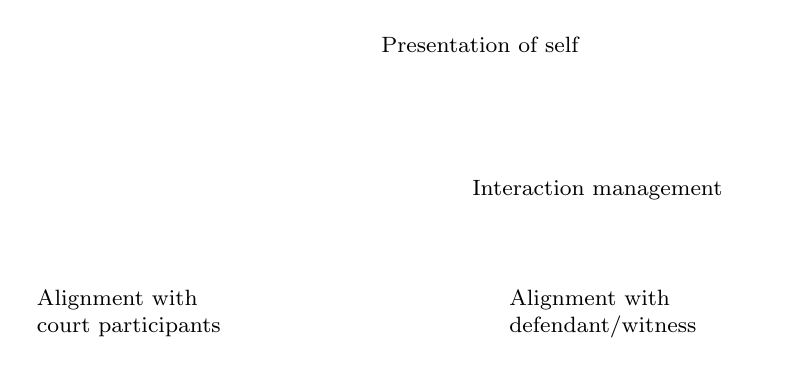
\begin{tikzpicture}
        [axisdesc/.style={font=\footnotesize,text width=2.5cm,align=left}]
        \devauxcos%definition is in localcommands.tex
\node [axisdesc,below]   at (xyz cs:x=-3)   {Alignment with court participants};
\node [axisdesc,below]   at (xyz cs:x=3)   {Alignment with defendant\slash witness};
\node [axisdesc,text width=2.75cm,right]   at (xyz cs:y=3)   {Presentation of self};
\node [axisdesc,text width=3.5cm,right,fill=white]   at (xyz cs:z=-3)   {Interaction management};
\end{tikzpicture}
\caption{\citegen{Llewellyn-Jones2014} role-space template\label{fig:devaux:1}}
\end{figure}

In order to design the interpreter’s role-space, \citeauthor{Llewellyn-Jones2011} (\citeyear[4--5]{Llewellyn-Jones2011}; \citeyear[62]{Llewellyn-Jones2013}) draw a sample list of criteria used to assess the court interpreter’s presentation of self, participant alignment, and interaction management, which are summarised in \tabref{tab:devaux:1}. 

\begin{table}
\resizebox{\textwidth}{!}{%
\begin{tabularx}{1.2\textwidth}{QQQ}
\lsptoprule
Presentation of Self & Interaction Management & Participant Alignment\\\midrule
The interpreter...\\
introduces herself\slash takes the oath or affirms & requests for clarification or repetition & addresses specific participants directly\\
\tablevspace
refers to herself as “the interpreter” & manages turn-taking & provides feedback and back-channels\\
\tablevspace
gives insights into her personal likes/dislikes & requests specific actions & explains some aspects of the interpreting process\\
\tablevspace
answers direct questions & requests change in the environment & smiles when a participant makes a humorous contribution\\
\tablevspace
divulges personal information about herself &  & reads body language\slash establishes eye-contact\\
\lspbottomrule
\end{tabularx}
}
\caption{\label{tab:devaux:1}Sample list of role-space criteria}
\end{table}
As an example which could illustrate \tabref{tab:devaux:1}, \citet[77--78]{Llewellyn-Jones2014} report on the role-space that they adopted whilst interpreting during a court hearing. Their presentation of self was low as they introduced themselves as the interpreters, and then they were sworn in, but they did not provide the other participants with any further information about themselves. Their interaction management was quite high as they could seek clarification, and they could ask for questions to be reframed. However, they were more reluctant to regulate the interaction between participants. Finally, their participant alignment was limited to ensuring participants’ understanding of the proceedings. As a result, they aligned equally between the participants, but they felt that their alignment was very low. Their role-space model is represented in \figref{fig:devaux:2}.

  
%%please move the includegraphics inside the {figure} environment
%%\includegraphics[width=\textwidth]{Ch4-img14.png}
 

\begin{figure}
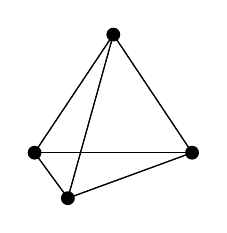
\begin{tikzpicture}
\devauxcos%see localcommands.tex
\def\devauxlist{x=-1,x=1,y=1.5,z=1.5}
\foreach \i in \devauxlist {
        \node[fill=black,circle,minimum size=5pt,inner sep=0pt] at (xyz cs:\i) {};
        \foreach \j in \devauxlist {
            \draw (xyz cs:\i) -- (xyz cs:\j);
        }
}
\end{tikzpicture}
\caption{\citegen{Llewellyn-Jones2014} role space model based on their court experience described above\label{fig:devaux:2}}
\end{figure}

\section{Methodology and research design}
\label{sec:devaux:4}
From a methodological viewpoint, this study was anchored within Actor-Net\-work Theory (\textsc{ant}). Such an approach enables researchers to examine human and non-human actors as forming part of an interactive network.\footnote{For more information on \textsc{ant}, \citet{Latour2005} offers a good introduction on the interaction and networks created between humans and non-human entities.} From an \textsc{ant} ontological viewpoint, reality stems from the interplay created between human and non-human actors, and epistemologically, reality may be plural and unravelling it “requires identifying and following those actually involved in [the network’s] creation” \citep[112]{Bonner2013}. Applying \textsc{ant} to this study enabled the researcher to examine how the interpreter, the other court participants, and the \textsc{vci} equipment interacted, through the eyes of the interpreter, to create a network during the court hearing within which the interpreter would express her role-space.\footnote{For more information on the extent to which \textsc{ant} and role-space are compatible, see \citet{Devaux2017b}.} 

After obtaining ethical approval from the University of Salford to carry out the doctoral project, 1,150 prospective participants who were all members of the National Register of Public Service Interpreters (\textsc{nrpsi}) were contacted by email in 2014. Thirty-nine expressed an interest and, in the end, eighteen practising court interpreters in England and Wales were interviewed. When applying \citegen{Seidman2006} principles of sufficiency and saturation of information, the number of participants was deemed sufficient. 

In terms of participants’ profiles, there were sixteen women and two men sharing, between them, a wide range of language combinations (mainly European languages, but also Arabic, Chinese, and Turkish). All participants had a Diploma in Public Service Interpreting (\textsc{dpsi}), or equivalent, which at the time was a requirement to become a court interpreter. Several participants had more than one qualification, and they often combined a \textsc{dpsi} with a degree or an MA in Languages or in Translation and Interpreting Studies. Most participants (twelve) had at least ten years’ experience in court interpreting. Their experience in interpreting in \textsc{vci} was somehow more limited with most participants having interpreted on 10 or fewer occasions in \textsc{vci a} and/or \textsc{b}.   

In line with the \textsc{ant}’s methodological stance, semi-structured interviews were conducted with the eighteen participants. The interview pointers were based on \tabref{tab:devaux:1} in order to ensure that enough information was collected so that a role-space model could be drawn for each participant. The interviews were conducted either face-to-face or via Skype.\footnote{For a more in-depth discussion on conducting interviews face-to-face or via Skype, see \citet{Devaux2017b}.} The recordings were then transcribed verbatim and coded using NVivo. The corpus gathered accounted for 12.5 hours of recording. 

\section{Data analysis through role-space}
\label{sec:devaux:5}
The eighteen participants taking part in this study expressed different role perceptions, and the results are summarised in Tables \ref{tab:devaux:2}, \ref{tab:devaux:3}, \ref{tab:devaux:4}, and \ref{tab:devaux:5}.

\begin{table}
\resizebox{\textwidth}{!}{%
\begin{tabular}{llll}
\lsptoprule
   & {Presentation of self} & Participant Alignment\footnote{The sign “>” designates the side towards which the interpreter aligned.} & {Interaction Management}\\\midrule
P1 & Very low & > Court & Very low\\
P3 & Low & > Court & Low\\
P5 & Low & Equal & High\\
P6 & Low & Equal & Quite high \\
P7 & Low & > Court & Low\\
P8 & Very low & > Court & From low to high\\
P9 & Low & > Court & High\\
P14 & Low & Equal & From low to high\\
P15 & Low & Equal & From very low to high\\
P16 & Low & > Court & From low to quite high\\
P17 & Low & > Court & Low\\
P18 & Low & > Court & Low to quite high\\
\lspbottomrule
\end{tabular}
}
\caption{Role-space in \textsc{vci a}\label{tab:devaux:2}}
\end{table}

\begin{table}
\resizebox{\textwidth}{!}{%
\begin{tabular}{llll}
\lsptoprule
& {Presentation of self} & {Participant Alignment} & {Interaction Management}\\\midrule
P1 & Very low & Equal & Low\\
P2 & Low & Equal & Low to quite high\\
P3 & Low & > Defendant & High\\
P4 & Low & > Witness & Quite high\\
P5 & Low & Equal & High\\
P6 & Low & Equal & Quite high \\
P11 & Low & > Witness & High\\
P15 & Low & Equal & Low to high \\
P16 & Low & > Witness & Low to quite high\\
P18 & Low & Equal & Low to quite high\\
\lspbottomrule
\end{tabular}
}
\caption{Role-space in \textsc{vci b}\label{tab:devaux:3}}
\end{table}

The reasons explaining this assessment are summarised below. However, as some participants’ models differed greatly from those presented in \tabref{tab:devaux:2} and \tabref{tab:devaux:3}, their models are discussed separately in \sectref{sub:devaux:5.4}. Due to word constraints and in light of the various role-spaces created, this section offers a brief summary of the data analysis, and a more in-depth analysis is provided in \citet{Devaux2017b}.

\subsection{Presentation of self}
In \textsc{vci a}, P1 and P8 could not introduce themselves and/or were not sworn-in when all parties were in attendance. P1 stated that she could have been “the cleaner, (…) the woman with the microphone.” Similarly, P8 believed that it was not obvious to the defendant that she was the interpreter. P1 added that she believed it was difficult for interpreters to be perceived as impartial as the defendant was on the other side of the screen. Similarly, in \textsc{vci b}, P1 stated the introduction/sworn-in process was missing. As such the presentation of self for these participants in these settings was deemed very low. 

The other participants reported that they had been sworn-in. They had introduced themselves, as the interpreter, to all the parties on both sides of the screen. Most also believed that impartiality was not impaired by the use of \textsc{vci} equipment. However, they did not divulge any further information, for instance about themselves. As such, their presentation of self was deemed low.

\subsection{Participant alignment}
Four participants in \textsc{vci a} and six in \textsc{vci b} reported that they were able to align equally between the participants on both sides of the screen. Although some reported that their ability to hear/see well may be slightly affected by the use of \textsc{vci} equipment, it had never been so poor that it had affected their interpreting performance. In fact, one participant (P15) even reported that it was easier to see/hear the court participants in \textsc{vci a} than when interpreting face-to-face from the dock. The participants were also able to replicate body language, give feedback, and intervene to explain cultural references, when needed. 

The other participants’ experience differed greatly. In \textsc{vci a}, they reported that they encountered technical difficulties that impacted on their ability to hear and/or see the remote party well. They often stated that the sound was echoing, and P1 even compared the setting to a mausoleum. Furthermore, they felt that they could not read the witness or defendant’s body language to obtain feedback or backchannel. Some also stated that the use of \textsc{vci} equipment had a negative impact on the proceedings as they could not interpret all the content, cultural references, and/or build a rapport with the defendant in \textsc{vci a} in order to adapt their terminology. Interestingly, the reason P9 aligned more towards the participants in court differs. She did not report on her inability to align with the defendant, but by sitting next to the judge, the close physical proximity made her over-align towards the participants in court. In \textsc{vci b}, participants stated that it was more difficult to replicate body language as the screens were too small. They also reported that although it was easier to build a relationship with the defendant/witness, it was more difficult to reproduce this with the participants in court. As a result, these participants aligned more towards the party with whom they were physically present. 

\subsection{Interaction management} 

Some participants perceived that their interaction management had been either very low, low, quite high, or high. Their reasons differed and are summarised below. 

P1 felt that her interaction management was very low in \textsc{vci a}. She argued that the defendant was so removed from the process that no interaction could take place. Other participants’ interaction management was low as they felt that the working environment was more daunting, and they were reluctant to interrupt the proceedings to ask for clarification. They also felt that the use of technology made the defendant less likely to interrupt the proceedings. On the other hand, some participants’ interaction management was high or very high, be it in \textsc{vci a} or \textsc{vci b}. For instance, P6 and P9 said that it was easier to ask for repetitions and clarification as they were in clear view of the judge in \textsc{vci a}. P9 also said that she always mentioned to the defendant that he could interrupt her at any time, if he did not understand. On several occasions, the defendant then interrupted her in \textsc{vci a}, and she was able to manage the flow of interaction. Similarly, P4’s interaction management in \textsc{vci b} was quite high. Although she did not encounter any instances of overlapping turns, she managed the interaction by asking the court to speak in “smaller chunks” as technology was used. Interestingly, she also stated that the defendant was less engaged in the proceedings, despite the interpreter being present in the same room. P5 managed the interaction by telling the defendant “Please don’t talk, I am listening”, and then she informed the court that the defendant had a question. In the same vein as P4’s approach, P5 required the court to speak one sentence at a time. 

The above participants’ interaction management could be described as static in the sense that they perceived it to be either very low, low, quite high, or high in \textsc{vci a\slash b}. Other participants perceived that their interaction management could be expressed alongside a continuum ranging from very low to high. These participants felt that there was no need/hardly any need to intervene during the \textsc{vci} court hearing, be it in \textsc{vci a} and/or \textsc{vci b}. Hence, their interaction management was very low/low. Nonetheless, had the need occurred, they stated that it would be possible to have a quite high/high interaction management, and that the use of \textsc{vci} technology would not impair their abilities to manage the interaction. The reasons put forward by the participants as to why interaction management in \textsc{vci} was very low/low differed, and they can be summarised as follows:
% \todo{converted from inline enumeration to list}

\begin{enumerate}
\item the hearings tend to be quite short, hence reducing the opportunity to encounter cultural references 
\item interpreter’s expectation that the defendant would show enough respect to the court not to intervene 
\item over-lapping turns tend to be more frequent at police stations 
\item as the defendant appears remotely, he is less likely to intervene in court 
\item the interventions were “quite clear and straightforward” (P15)
\end{enumerate}

It would not be feasible to create a role-space model for each of the participants in this article.\footnote{A detailed role-space analysis for each participant and their role-space model is available in \citet{Devaux2017b}.} However, the general shape of their models could be divided into two categories: those who perceived their interaction management as static, therefore creating a four-face-pyramid model (\figref{fig:devaux:3}), and those who perceived their interaction management as a continuum, thus forming a five-face-pyramid one (\figref{fig:devaux:4}).  
 

\begin{figure}[p]
	%%please move the includegraphics inside the {figure} environment
	%%\includegraphics[width=\textwidth]{Ch4-img15.png}
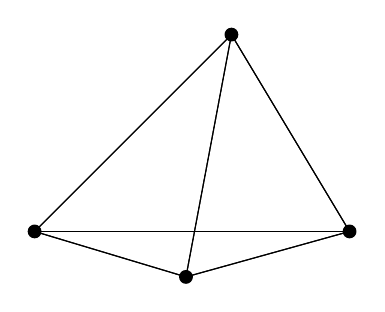
\begin{tikzpicture}
\def\devauxlist{x=-2.5,x=1.5,y=2.5,z=1.5}
\devauxcos%see localcommands.tex
\foreach \i in \devauxlist {
        \node[fill=black,circle,minimum size=5pt,inner sep=0pt] at (xyz cs:\i) {};
        \foreach \j in \devauxlist {
            \draw (xyz cs:\i) -- (xyz cs:\j);
        }
}
\end{tikzpicture}
\caption{P9's four-shape model in \textsc{vci a}\label{fig:devaux:3}}
\end{figure}

\begin{figure}[p]
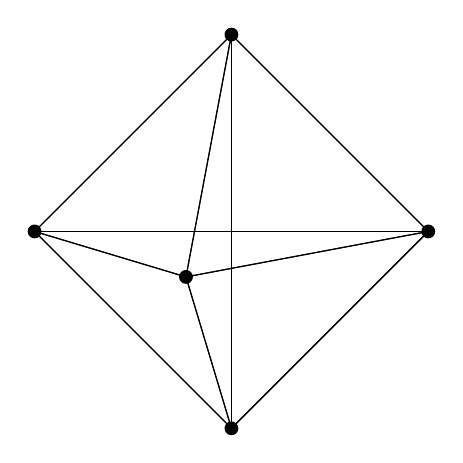
\begin{tikzpicture}
\def\devauxlist{x=-2.5,x=2.5,y=2.5,y=-2.5,z=1.5}
\devauxcos%see localcommands.tex
\foreach \i in \devauxlist {
        \node[fill=black,circle,minimum size=5pt,inner sep=0pt] at (xyz cs:\i) {};
        \foreach \j in \devauxlist {
            \draw (xyz cs:\i) -- (xyz cs:\j);
        }
}
\end{tikzpicture}
	%%please move the includegraphics inside the {figure} environment
	%%\includegraphics[width=\textwidth]{Ch4-img16.png}
\caption{P15's five-face pyramid shape model in \textsc{vci a}\label{fig:devaux:4}}
\end{figure}

\subsection{Split role-space}
\label{sub:devaux:5.4}
Finally, some interpreters created one role-space for the participants in court and another one for defendant and witness. Their role-space axes are summarised in Tables~\ref{tab:devaux:4} and \ref{tab:devaux:5}. 

\begin{table}[t]
\resizebox{\textwidth}{!}{%
\begin{tabular}{llllll}
	\lsptoprule
	& \multicolumn{2}{c}{Presentation of self } & Participant Alignment & \multicolumn{2}{c}{Interaction management} \\ \cmidrule(lr){2-3}\cmidrule(lr){5-6}
& Court & Defendant &  & Court & Defendant\\
\midrule
P10 & Low & Very low & > Court & High & Quite high\\
P12 & Low & Very low & Equal & \multicolumn{2}{l}{Low to quite high}\\
\lspbottomrule
\end{tabular}
}
\caption{Split role-space in \textsc{vci a}\label{tab:devaux:4}}
\end{table}

\begin{table}[t]
\resizebox{\textwidth}{!}{%
\begin{tabular}{llllll}
\lsptoprule
& \multicolumn{2}{c}{Presentation of self } & Participant Alignment & \multicolumn{2}{c}{Interaction management} \\ \cmidrule(lr){2-3}\cmidrule(lr){5-6}
& Court & Defendant &  & Court & Defendant\\ \midrule

P13 & Very low & Low & > Defendant and solicitor & Very low & Quite high\\
P14 & Very low & Low & Equal & \multicolumn{2}{l}{Low to quite high} \\
P17 & Very low & Low & Equal & \multicolumn{2}{l}{Low to high}\\
\lspbottomrule
\end{tabular}
}
\caption{Split role-space in \textsc{vci b}\label{tab:devaux:5}}
\end{table}


The reasons justifying the above participants’ alignment are similar to those mentioned previously. Therefore, they will not be analysed again, and this sub-section will focus on their presentation of self and/or interaction management.\largerpage[-2]

In \textsc{vci a} and \textsc{vci b} their presentation of self was low with the co-located party, and very low with the remote participant(s). They could introduce themselves as the court interpreter with their co-located party. However, they could not replicate the process with the remote party, or even be sworn-in, for instance. Also, P12 raised some concerns on how she could be perceived as impartial by the defendant in \textsc{vci a} as she was seen “on the same side” of the court, and P13 thought it was more difficult to establish an atmosphere of trust with the participants in court in \textsc{vci b}. Hence, their presentation was low with the co-located party and very low with the remote participant(s).

P12 in \textsc{vci a}, and P14 and P17 in \textsc{vci b} perceived their interaction management alongside a continuum ranging from low to quite high/high. Again, the reasons were similar to those for the participants above, so they will not be discussed here. 

The interaction management for P10 in \textsc{vci a} and P13 in \textsc{vci b} differed between the participants in court and the remote defendant/witness. P10 believed that the use of \textsc{vci} equipment did not impact on his ability to manage the interaction with the participants in court. Yet, P10’s interaction management with the other side was lower as “giving the conversation a rhythm [had been] much more difficult” (P10) with the defendant. Similarly, P13’s interaction management was very low with the participants in court. Although he had encountered difficulties hearing parts of the court interventions, he did not intervene to notify the participants in court of the issue. Nevertheless, his interaction management with the solicitor and the defendant was quite high as they were sitting together, and he could attract their attention, and ask them for repetitions/clarification.

As a result, these participants’ role-space model was split, and their shapes differed greatly from the other participants, as illustrated by Figures 5 (P10), 6 (P12), 7 (P13), 8 (P14), and 9 (P17). Worth noting is that P12 in \textsc{vci a} and P14 and P15 in \textsc{vci b} created two \textsc{3d} role-space models. In order to preserve their model’s readability, it was decided to split them into two graphs: one representing her role-space model with the participants in court (on the left hand-side), and one with the defendant (on the right-hand side).

  

 

\begin{figure}
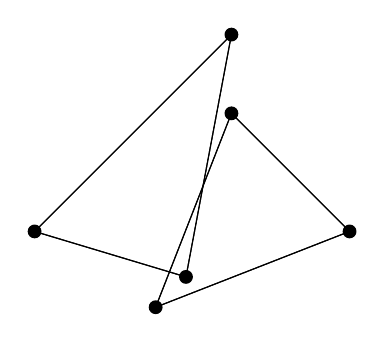
\begin{tikzpicture}
\devauxcos%see localcommands.tex
\def\devauxlist{x=-2.5,y=2.5,z=1.5}
\foreach \i in \devauxlist {
        \node[fill=black,circle,minimum size=5pt,inner sep=0pt] at (xyz cs:\i) {};
        \foreach \j in \devauxlist {
            \draw (xyz cs:\i) -- (xyz cs:\j);
        }
}
\def\devauxlist{x=1.5,y=1.5,z=2.5}
\foreach \i in \devauxlist {
        \node[fill=black,circle,minimum size=5pt,inner sep=0pt] at (xyz cs:\i) {};
        \foreach \j in \devauxlist {
            \draw (xyz cs:\i) -- (xyz cs:\j);
        }
}
\end{tikzpicture}
	%%please move the includegraphics inside the {figure} environment
	%%\includegraphics[width=\textwidth]{Ch4-img17.png}
\caption{P10's role-space model in \textsc{vci a}}
\end{figure}


  
%%please move the includegraphics inside the {figure} environment
%%\includegraphics[width=\textwidth]{Ch4-img18.png}
   
%%please move the includegraphics inside the {figure} environment
%%\includegraphics[width=\textwidth]{Ch4-img19.png}
 


\begin{figure}
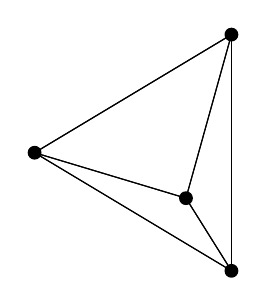
\begin{tikzpicture}
\devauxcos%see localcommands.tex
\def\devauxlist{x=-2.5,y=1.5,y=-1.5,z=1.5}
\foreach \i in \devauxlist {
        \node[fill=black,circle,minimum size=5pt,inner sep=0pt] at (xyz cs:\i) {};
        \foreach \j in \devauxlist {
            \draw (xyz cs:\i) -- (xyz cs:\j);
        }
}
\end{tikzpicture}
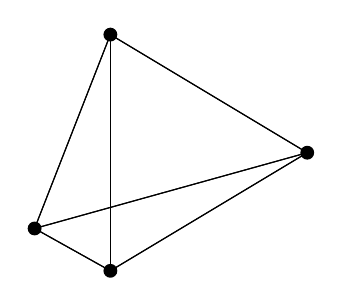
\begin{tikzpicture}
\devauxcos%see localcommands.tex
\def\devauxlist{x=2.5,y=1.5,y=-1.5,z=2.5}
\foreach \i in \devauxlist {
        \node[fill=black,circle,minimum size=5pt,inner sep=0pt] at (xyz cs:\i) {};
        \foreach \j in \devauxlist {
            \draw (xyz cs:\i) -- (xyz cs:\j);
        }
}
\end{tikzpicture}
\caption{P12’s role-space model with the court (left) and the defendant (right) in \textsc{vci a}}
\end{figure}

  
%%please move the includegraphics inside the {figure} environment
%%\includegraphics[width=\textwidth]{Ch4-img20.png}
 

\begin{figure}
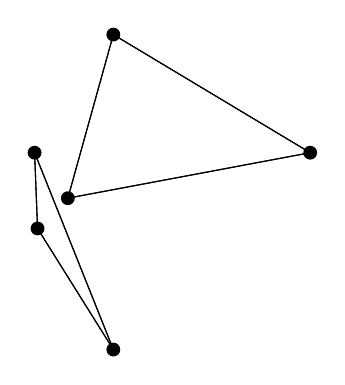
\begin{tikzpicture}
\devauxcos%see localcommands.tex
\def\devauxlist{x=-1,y=-2.5,z=2.5}
\foreach \i in \devauxlist {
        \node[fill=black,circle,minimum size=5pt,inner sep=0pt] at (xyz cs:\i) {};
        \foreach \j in \devauxlist {
            \draw (xyz cs:\i) -- (xyz cs:\j);
        }
}
\def\devauxlist{x=2.5,y=1.5,z=1.5}
\foreach \i in \devauxlist {
        \node[fill=black,circle,minimum size=5pt,inner sep=0pt] at (xyz cs:\i) {};
        \foreach \j in \devauxlist {
            \draw (xyz cs:\i) -- (xyz cs:\j);
        }
}
\end{tikzpicture}
\caption{P13's role-space model in \textsc{vci b}}
\end{figure}

  
%%please move the includegraphics inside the {figure} environment
%%\includegraphics[width=\textwidth]{Ch4-img21.png}
   
%%please move the includegraphics inside the {figure} environment
%%\includegraphics[width=\textwidth]{Ch4-img22.png}
 

\begin{figure}
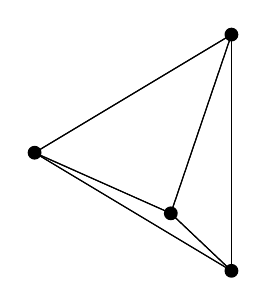
\begin{tikzpicture}
\devauxcos%see localcommands.tex
\def\devauxlist{x=-2.5,y=1.5,y=-1.5,z=2}
\foreach \i in \devauxlist {
        \node[fill=black,circle,minimum size=5pt,inner sep=0pt] at (xyz cs:\i) {};
        \foreach \j in \devauxlist {
            \draw (xyz cs:\i) -- (xyz cs:\j);
        }
}
\end{tikzpicture}
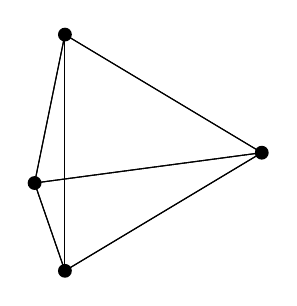
\begin{tikzpicture}
\devauxcos%see localcommands.tex
\def\devauxlist{x=2.5,y=1.5,y=-1.5,z=1}
\foreach \i in \devauxlist {
        \node[fill=black,circle,minimum size=5pt,inner sep=0pt] at (xyz cs:\i) {};
        \foreach \j in \devauxlist {
            \draw (xyz cs:\i) -- (xyz cs:\j);
        }
}
\end{tikzpicture}
\caption{P14's role-space with the participants in court (left) and the witness (right) in \textsc{vci b}}
\end{figure}

\begin{figure}
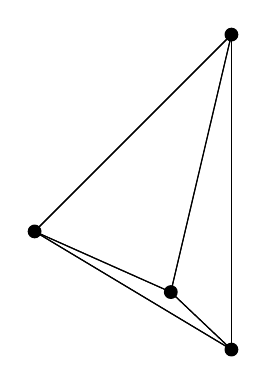
\begin{tikzpicture}
\devauxcos%see localcommands.tex
\def\devauxlist{x=-2.5,y=2.5,y=-1.5,z=2}
\foreach \i in \devauxlist {
        \node[fill=black,circle,minimum size=5pt,inner sep=0pt] at (xyz cs:\i) {};
        \foreach \j in \devauxlist {
            \draw (xyz cs:\i) -- (xyz cs:\j);
        }
}
\end{tikzpicture}
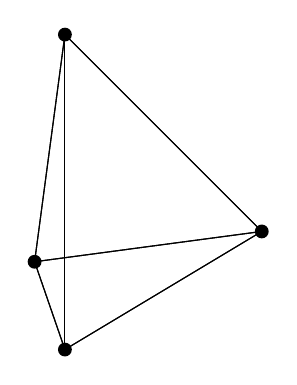
\begin{tikzpicture}
\devauxcos%see localcommands.tex
\def\devauxlist{x=2.5,y=2.5,y=-1.5,z=1}
\foreach \i in \devauxlist {
        \node[fill=black,circle,minimum size=5pt,inner sep=0pt] at (xyz cs:\i) {};
        \foreach \j in \devauxlist {
            \draw (xyz cs:\i) -- (xyz cs:\j);
        }
}
\end{tikzpicture}
%%please move the includegraphics inside the {figure} environment
%%\includegraphics[width=\textwidth]{Ch4-img23.png}
   
%%please move the includegraphics inside the {figure} environment
%%\includegraphics[width=\textwidth]{Ch4-img24.png}
\caption{\label{fig:devaux:15}P17's role-space model with the participants in court (left) and the defendant (right) in \textsc{vci b}}
\end{figure}

The participants perceived their role differently in \textsc{vci a} and/or \textsc{b}, and, in fact, very few participants shared the exact same role-space (except, for instance, P3 and P7 in \textsc{vci a}, and P12 in \textsc{vci a} and P14 in \textsc{vci b}). Although there were many different perceptions, their role-space can be grouped into three main categories: a fixed, a continuum, or a split role-space. Also, the use of equipment affected the participants’ axes to various extents, and the distance between the participants meant that some interpreters were not always able to present themselves, manage aspects of the interaction, and/or align equally between the court participants. Worth noting is the fact that some participants mentioned that such equipment could also improve parts of the court proceedings. Notably, it was easier for some interpreters to seek clarification in \textsc{vci a}. 

\section{Discussion of findings}
\label{sec:devaux:6}
Building on the above findings, this section discusses the participants’ perceptions of their role in light of the literature review, and it suggests some recommendations for training.

\subsection{True-to-life experience}

\Citet{vanRotterdam2011} argue that the use of \textsc{vci} equipment cannot represent a true-to-life experience due to various factors affecting the proceedings (such as potential poor quality of sound/picture, establishing eye contact, participants’ reactions/interactions, etc.). In this study, parts of the data confirm that the absence of body language and back channelling, for instance, were highlighted as factors affecting some participants’ experience, and these findings align with other studies which analyse the impact of the use of technologies. For instance, \citet{Radburn-Remfry1994} argues that, in a mono-lingual setting, participants in court may feel more emotionally detached from the defendant during \textsc{vci} hearings. \citet{Hodges2008} raises questions regarding the working relations between the defendant and the defence counsel. Supporting their studies, P1 felt that the defendant had not been taking part in his own hearing as he was too divorced from the proceedings. P1 believed that at this point, the right to see due legal process taking place could be questioned. This would support the idea that \textsc{vci} cannot replicate a true-to-life experience. It is worth noting that the participants’ experience was not homogeneous, and it was even contradictory in some parts. For instance, P9 believed that when the defendant did not speak with a strong regional accent, there were no differences regarding whether the hearing was conducted in face-to-face or \textsc{vci a} mode. This plurality of interpreters’ perceptions reflects this study’s epistemological stance and the interpreters’ multivocality. The array of perceptions is a window opening onto the actors’ various realities, which suggests that a true-to-life experience can be a rather subjective notion, and from the interpreters’ viewpoints \textsc{vci} equipment can impair or improve aspects of \textsc{vc}-conducted court hearing.

\subsection{Factors affecting the interpreter’s perception of her role}
The interpreters’ different role perceptions in this study are not a new phenomen\-on. Some studies in \textsc{is} offer several factors justifying the interpreters’ perceptions of their role differently in face-to-face settings, such as qualifications \citep{Martin2008} and cultural acceptability \citep{Merlini2009}. One could also question the extent to which professional experience shape the interpreters’ perceptions. All the participants in this study were \textsc{dpsi} qualified -- some passed the same type of \textsc{dpsi} (e.g. law), and some were trained in the same centres. Yet, their role-spaces were different. Furthermore, some participants shared the same culture, but their role-space models differed. Finally, P1 and P2 in \textsc{vci b} have many years of experience as court interpreters (20 and 15 years, respectively), but their role-spaces also differ. Similarly, P6 and P10 have both interpreted over ten times in \textsc{vci}, but the role-spaces created are different. This tends to suggest that if qualification, cultural acceptability, and professional experience influence the participants’ role perception in this study, these could only be factors partly contributing to shaping such perceptions. Nevertheless, the recurring denominator when analysing the interviews seems to be the extent to which the participants felt that the use of \textsc{vci} equipment had limited parts of their role-space. 

Due to the use of \textsc{vci} equipment, some participants had a very low presentation of self as they could not introduce themselves and/or be sworn-in. In her study, \citet{Fowler2013} observed that some interpreters were not introduced at the start of the hearing. In such instances, there was “a tendency for the interpreter to defer to the court in matters which were properly part of their own professional remit” \citep[245]{Fowler2013}. P1 raised the sitting arrangement as a potential issue with being perceived as impartial. This has been identified as a potential issue in the Avidicus 2’s research report, where their findings show that “the seating arrangements gave the impression that the participants on one side of the video link spoke ‘as one’ or ‘could be perceived as one’” \citep[53]{Braun2013}. However, it is worth noting that other participants perceived that the seating arrangement was in fact improving aspects of their role-space as they were no longer interpreting from the dock at the back of the courtroom.

Some participants also aligned more towards one party as they felt that the technical difficulties encountered, and/or the lack of feedback or back-channell\-ing opportunities, had not enabled them to establish a rapport with the court participant(s) on the other side of the screen. As a result, their participant alignment with the remote party had been lower. These findings align with \citegen{Rombouts2011} and \citegen{Napier2011} studies, which reveal that it is more difficult to establish a rapport with the remote party, or with \citeauthor{Braun2016b} (\citeyear[4]{Braun2016b}), who asserts that \textsc{vci} “entail[s] a reduction in the quality of the intersubjective relations between the participants.” This study also shows that when the interpreters’ participant alignment differs between actors, there had been a greater tendency to align towards the participants in court, rather than the witness or, to even a lesser extent, the defendant. Although the findings partly corroborate the difficulty to establish a rapport with the remote party, they also suggest that there are alignment disparities between the court actors and, amongst all the participants, the defendant is the party that the interpreter may be the least willing to over-align towards.

Finally, a few participants believed that the use of \textsc{vci} equipment had slightly reduced their interaction management, but overall it had remained quite high, which is similar to \citegen{Llewellyn-Jones2014} experience as court interpreters. Other participants had a high interaction management, whilst others had perceived it as ranging from low to high. Only a few participants had felt that their interaction management had been low. To some extent, the data gathered in this study concurs partially with the literature review, in the sense that court interpreters have to manage the interaction by giving turns, for instance \citep{Angelelli2003,Llewellyn-Jones2014,Martin2008}, and they have to do so even more when technologies are used, to the extent that they become fully-fledged independent actors \citep{Lee2007,Rosenberg2007}. Similarly, \citet{Braun2016a} argues that the discourse is more fragmented in \textsc{vci}-conducted legal proceedings, and it is therefore not surprising that many participants had a quite high or high interaction management. What remains unclear, though, is the reason why some court interpreters failed to intervene in order to re-balance their interaction management. 

The use of \textsc{vci} equipment affected the participants’ axes to varying degrees and very few participants’ role-space was similar to 
% \todo{Do you want to cite the authors here only, or also the specific 2014 publication?}
\citegen{Llewellyn-Jones2014} court experience (\figref{fig:devaux:2}). Despite such differences the shapes of most participants’ role-space models were similar to the types discussed in \citegen{Llewellyn-Jones2014} work. Indeed, some interpreters perceived their role as a \textsc{3d} fixed entity, whilst other created a \textsc{3d} continuum. However, unlike \citegen{Llewellyn-Jones2014} models in face-to-face settings, this study reveals that the interpreter can adopt a third type of model, whereby she splits her role-space into two sub-spaces. In these instances, this study’s participants felt that the use of technology had a limited impact on their role perceptions with their co-located party, but it restricted aspects of their role-space with the remote party. 

\subsection{Recommendations for training}
As mentioned by some participants and as confirmed when examining the \citegen{IoL2015} \textit{Handbook for Candidates} sitting the \textsc{dpsi} examination, it seems that \textsc{vci} training does not form an integral part of the \textsc{dpsi} curriculum. Therefore, given the fact that \textsc{vci} is used in court, and given the impact that the equipment can have on the interpreter’s perception of her role, it is recommended that training in the use of \textsc{vci} in court be offered.  

In order to ensure that prospective court interpreters possess more than a conceptual understanding of \textsc{vci}, \textsc{dpsi} centres should give students the opportunity to observe proceedings taking place in both \textsc{vci a} and \textsc{b} modes. It is also important that trainees are given the opportunity to practise role-plays in these two modes. Although centres may not be equipped with \textsc{vci} technologies meeting the \citegen{TelecommunicationUnion2009} H323 Recommendation, trainees could nonetheless practise role-plays using cruder technologies such as Skype. Furthermore, the aim of this article was not to develop or assess a curriculum for trainee \textsc{psi}s. However, centres could usefully develop resources based on the \citet{Braun2011c} or Avidicus 3 training outline. 

Participants also reported that court actors sometimes lack etiquette in terms of \textsc{vci} equipment and its use, making it more difficult for the interpreter to hear the proceedings. For instance, court staff or members of the public would leave the courtroom mid-hearing, court members would rustle papers near their microphone, or they would not speak in their microphone. Therefore, it is essential that legal practitioners also receive training in using \textsc{vci} equipment. Such training would need to make specific reference to conducting a bilingual \textsc{vci} hearing in the presence of an interpreter. As mentioned by some interpreters, training should not take place independently from the other participants, but rather all the court participants should also jointly train in using \textsc{vci} equipment. This confirms the recommendations put forward by other scholars such as \citet{Braun2011a} and \citet{Fowler2012}. 

It is worth noting that such training may also be relevant to practising court interpreters. The \textsc{nrpsi} has more than 2,000 registrants who are dispersed over a large geographical zone. A means to ensure that they are trained in \textsc{vci} mode could be for the \textsc{nrpsi} to offer \textsc{cpd} sessions to its members on this interpreting mode. 

\section{Conclusions}
\label{sec:devaux:7}
This article reported on the findings arising from \citegen{Devaux2017b} doctoral thesis. Based on the analysis of eighteen interviews conducted with court interpreters in England and Wales, it emerged that the interpreters perceived their role differently in \textsc{vci}, and they created different role-space models. The use of \textsc{vci} equipment affected various aspects of their presentation of self, participant alignment, and/or interaction management. Given the increasing use of \textsc{vci} equipment in court, this article also made some recommendations for training court interpreters. Although this study includes some limitations (e.g. a limited number of participants, who were all \textsc{dpsi} qualified), it paves the way to avenues for further research. To give a more generic picture of the court interpreter’s role, this study’s findings could be complemented by recruiting court interpreters without a \textsc{dpsi} (or equivalent). Another avenue to complement this study would be to observe court interpreters’ role when \textsc{vci} is used, and to interview the other court participants so that the impact of the interpreter’s role in \textsc{vci} could be examined. Furthermore, role-space is a relatively new theoretical framework and, as such, it would benefit from further empirical studies across various settings. Finally, it emerges from this study that some interpreters created a split-role model. The effect that this new model may have on the court participants and on the overall interaction is unknown and it would deserve further exploration. 

{\sloppy\printbibliography[heading=subbibliography,notkeyword=this]} 
\end{document}
